\subsection{Case 1: Scipion at CNB}
The National Center for Biotechnology (\cnb) forms part of the Spanish National Research Council (CSIC), the largest public research institution in Spain. 
The \cnb Cryo-Electron Microscopy Facility is a joint effort of the Nacional Center for Biotechnology and the Biological Research Centers. %The mission of the facility is to provide researchers access to the latest cryo-EM technology for high resolution imaging. 

This section in divided in two parts. In the first one we discuss the network setup that allows us to move the data from the microscope to the user laboratory. Then,  we comment on an additional software called  \emadmin. \emadmin has been specifically designed for the \cnb facility, it connects \scipion with the microscope acquisition software (\epu) and records the facility activity.

\subsubsection{Network Setup and IT Infrastructure}

At the beginning \cnb networking setup was a quite straightforward one, movies were stored in the same machine that ran \scipion and processed data were saved to external USB hard disks by this same machine. The situation changed when the new Falcon-III detector was installed. After that, data were produced at sustained speeds as high as 90 MB/sec (when acquiring four movies by hole in linear mode) and the main problem became to move smoothly the data through the entire pipeline from the microscope to the final user laboratory. In the following we describe such a pipeline (see \ffigure{fig:cnbpipeline} for details.).

\begin{figure}
  \centering
      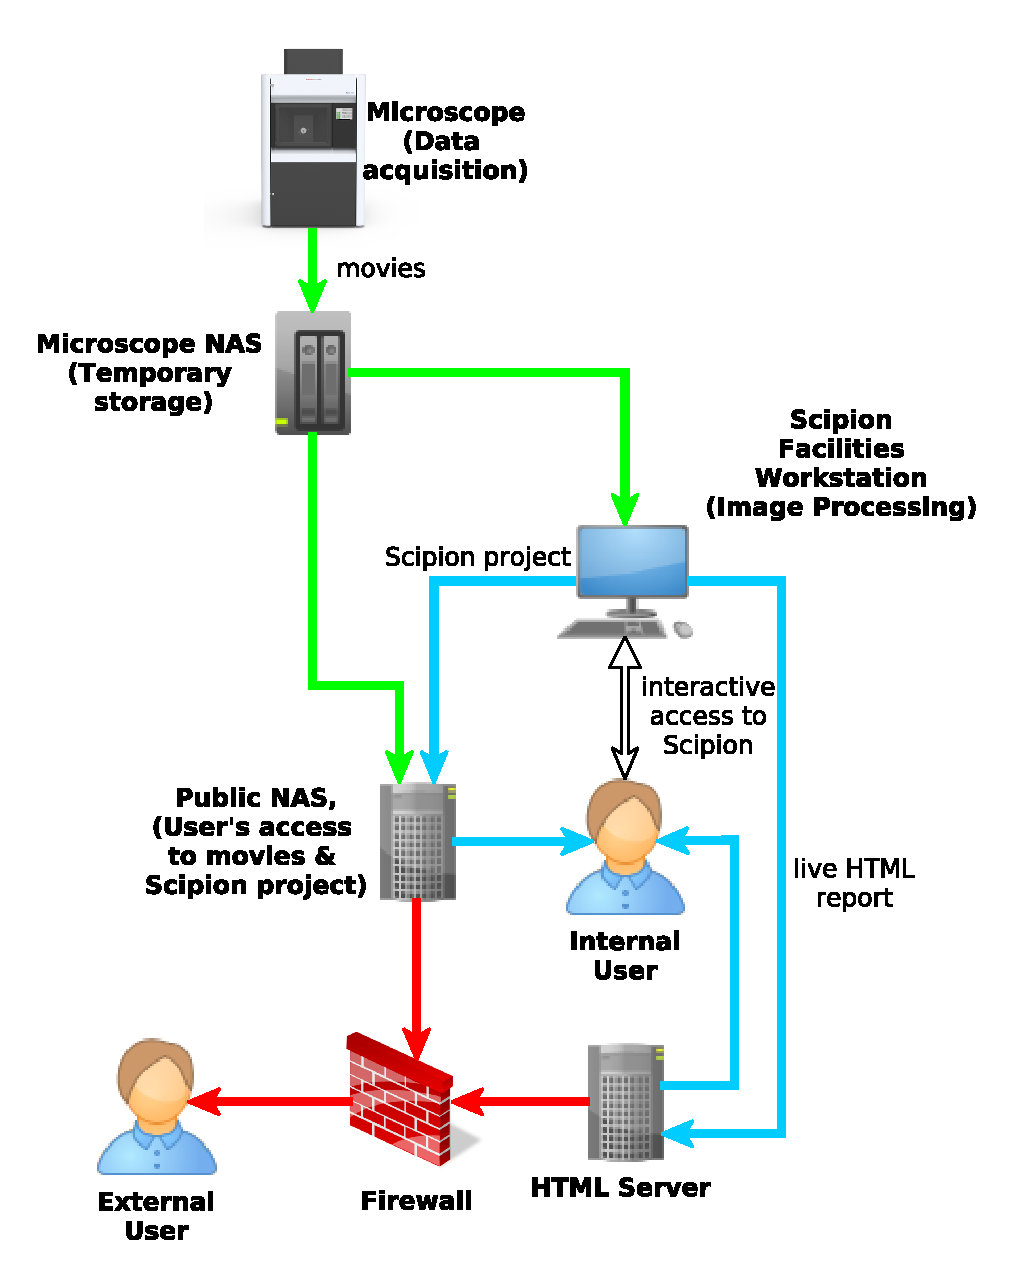
\includegraphics[width=0.75\textwidth]{images/diagram.pdf}
  \caption{Graphical representation of the data flow through the CNB facility. Green, blue and red lines represent the microscope private network, the \cnb local area network and the public (WAN) network respectively.}
  \label{fig:cnbpipeline}

\end{figure}

%From a network point of view there are three different levels of accessibility (see  \ffigure{fig:cnbpipeline}): (1) a private network that cannot be accessed by regular users -green lines in \ffigure{fig:cnbpipeline}-, (2) the \cnb LAN (local area network)  that can be accessed by any user who works inside the hosting  institution -blue lines in \ffigure{fig:cnbpipeline}- and (3) finally, there are two computers that may be accessed from outside the institution -red lines in \ffigure{fig:cnbpipeline}-, these computers give access to data and a web site respectively.

Data sets are recorded using \epu. The microscope control system has a 70 TB NAS (Network-attached storage) unit for saving movies as they are obtained (we will refer to this NAS as \mnas). This storage unit is shared through a Samba share and connected to the microscope private network using a 10Gb connexion. \scipion is executed on a Linux server which has two 1Gb NICs (network interface controllers) that connect it to the private network and the LAN (local area network) respectively (we will refer to this machine as \scipionbox). \scipionbox has 32 CPUs at 2.40GHz, 62 Gb of RAM memory and 2 \textit{Quadro M4000} GPUs. Finally, a second NAS with four 1Gb NICs is linked to the private, LAN and WAN networks (we will refer to this second NAS as \onas) so it can retrieve data from any computer and serve it to external users.

The data flow is as follows: (a) the microscope system stores movies in the \mnas, (b) when executing movie-alignment protocols \scipionbox reads the movies from the \mnas but does not store them locally, (c) \onas has access to \mnas and \scipionbox hard disks (d) \onas has a collection of scripts than may be used to incrementally backup \scipion projects and the associated movies to a local or remote disk, or serve this information through the Internet, and (e) in parallel, periodically \scipionbox transfers to  \hserver reports that may be checked by users or staff with an HTML browser (see a report example at \url{http://nolan.cnb.csic.es/scipionbox/lastHTMLReport/}).  

Although \cnb staff try to discourage the use of external USB hard disks versus network as way of retrieving the raw and processed data, this is the preferred option for most users.
USB 3.0 drives can theoretically handle data flows of 300 MB/s, but \cnb experience is that, in this busy environment, many of them  have trouble exceeding 50 MB/s. In most cases, 50 MB/s is enough to transfer the data before the following microscope  turn-shift starts. %When two, or even three, users try to download their
%data simultaneously, \onas works as front-end and isolates the data
%acquiring and processing infrastructure from the user's downloading activities.
Network users access to \onas using a hardened common account. This account only allows rsync connections and make impossible to retrieve data if the name of the project to be downloaded is unknown. %The achievable speed of copying a file depends on quite a few different factors 
%including the selected ciphers (algorithms for performing data encryption or decryption). Weak ciphers (as arcfour) have been activated in \onas to speed up transfer.

\subsubsection{Additional Software Developments: \emadmin}

\emadmin was born as a script that created a normalized tree of directories  
where movies acquired by the microscope could be stored, helped users to choose between a few predetermined image processing workflows and finally launched \scipion. At present it has grown in a client-server application that, in addition to the old script capabilities, has incorporated the following functions:

\begin{enumerate}
 \item Transparent addition of new workflows. \scipion is able to export any executed workflow as a json file. \emadmin can import this file and use it to create new predetermined workflows.
 \item  Automatic creation of pdf user's report that contains microscope acquisition parameters and histograms summarizing data resolution and defocus. 
 \item The above mentioned information is stored in a database for further analysis. By default, the system plots the  average resolution and astigmatism of the different acquisitions versus time.
 \item Remote management. \emadmin is a client server application, the client maybe executed in a machine different from the one that executes \scipion.
 \item Automatic backup of the \scipion project.
 \item \scipion is able to create live HTML reports on the image acquisition process. \emadmin keeps track of all of them and facilitates the access to this information.
\end{enumerate}

\emadmin is free software available at github repository (\url{https://github.com/rmarabini/webservices/tree/master/EMadmin}). The software can be freely downloaded and customized to meet the specific requirements of client organizations.

